\documentclass[11pt,a4paper]{report}
\usepackage[a4paper,margin=24mm,headheight=14pt]{geometry}
\usepackage[T1]{fontenc}
\usepackage[utf8]{inputenc}
\usepackage{lmodern}
\usepackage{amsmath}
\usepackage{graphicx}
\usepackage{xcolor}
\usepackage{booktabs}
\usepackage{tabularx}
\usepackage{longtable}
\usepackage{float}
\usepackage{caption}
\usepackage{fancyhdr}
\usepackage[hidelinks]{hyperref}
\usepackage{enumitem}
\usepackage{url}

\definecolor{ink}{RGB}{32,44,58}
\definecolor{accent}{RGB}{37,96,151}

\pagestyle{fancy}
\fancyhf{}
\fancyhead[L]{\textcolor{ink}{Qwen2.5-VL-3B Fine-Tuning}}
\fancyhead[R]{\textcolor{ink}{\thepage}}
\renewcommand{\headrulewidth}{0.4pt}

\graphicspath{{../../comparison/output/qwen25vl_finetuning/}}

\title{\textbf{Qwen2.5-VL-3B Fine-Tuning Case Study}\\[8pt]
Fashion-MNIST Baseline and LoRA Comparison}
\author{Analysis of repository evaluation artifacts}
\date{}

\begin{document}
\pagenumbering{roman}
\maketitle
\clearpage
\pagenumbering{arabic}

\chapter{Fine-Tuning Results}

\noindent
MNIST is a standard teaching example for neural networks, notably in
3Blue1Brown's
\href{https://www.youtube.com/watch?v=aircAruvnKk}{visual introduction to neural
networks} and throughout much of Michael Nielsen's open book
\href{https://neuralnetworksanddeeplearning.com/}{\emph{Neural Networks and Deep
Learning}}. The overlap is not coincidental: Nielsen's book was one of the
resources Grant Sanderson used to learn the subject before producing the video.
Fashion-MNIST preserves the same compact classification format while replacing
digits with clothing images.

\section{Experimental Question}

This case study asks whether parameter-efficient fine-tuning improves
Qwen2.5-VL-3B-Instruct on Fashion-MNIST. It compares:

\begin{itemize}[leftmargin=*]
    \item the unmodified Qwen2.5-VL-3B-Instruct baseline;
    \item the original Fashion-MNIST LoRA adapter;
    \item the balanced Fashion-MNIST LoRA adapter.
\end{itemize}

Each artifact contains the same 50 ordered test examples, enabling paired
analysis. Fine-tuning used 100 training and 20 validation examples with seed
42. The adapters use 4-bit QLoRA on the query, key, value, and output
projections; the training defaults are two epochs and a learning rate of
\(10^{-4}\).

\section{Analysis Procedure}

The repository comparison schema and telemetry conventions are extended by
\path{comparison/compare_qwen25vl_finetuning.py}. It calculates accuracy,
macro and per-class metrics, confusion matrices, paired outcome changes,
McNemar's exact test, a 50,000-resample paired bootstrap, and inference
telemetry.

\section{Overall Classification Performance}

\begin{table}[H]
\centering
\small
\begin{tabular}{@{}lrrrrr@{}}
\toprule
\textbf{Model} &
\textbf{Correct} &
\textbf{Accuracy} &
\textbf{95\% CI} &
\textbf{Macro recall} &
\textbf{Macro F1} \\
\midrule
Baseline
& 19/50 & 0.380 & [0.259, 0.518] & 0.368 & 0.342 \\
Original LoRA
& 19/50 & 0.380 & [0.259, 0.518] & 0.349 & 0.296 \\
Balanced LoRA
& \textbf{24/50} & \textbf{0.480} & [0.348, 0.615]
& \textbf{0.455} & \textbf{0.455} \\
\bottomrule
\end{tabular}
\caption{Aggregate Fashion-MNIST performance on the common 50-image test
sample. Confidence intervals are Wilson intervals for accuracy.}
\label{tab:finetuned-overall}
\end{table}

The original adapter matches the baseline's 38\% accuracy but lowers macro F1
from 0.342 to 0.296. The balanced adapter reaches 48\% accuracy and 0.455 macro
F1. This is a 10-point accuracy gain and a 16.1\% relative reduction in errors.

\begin{figure}[H]
\centering
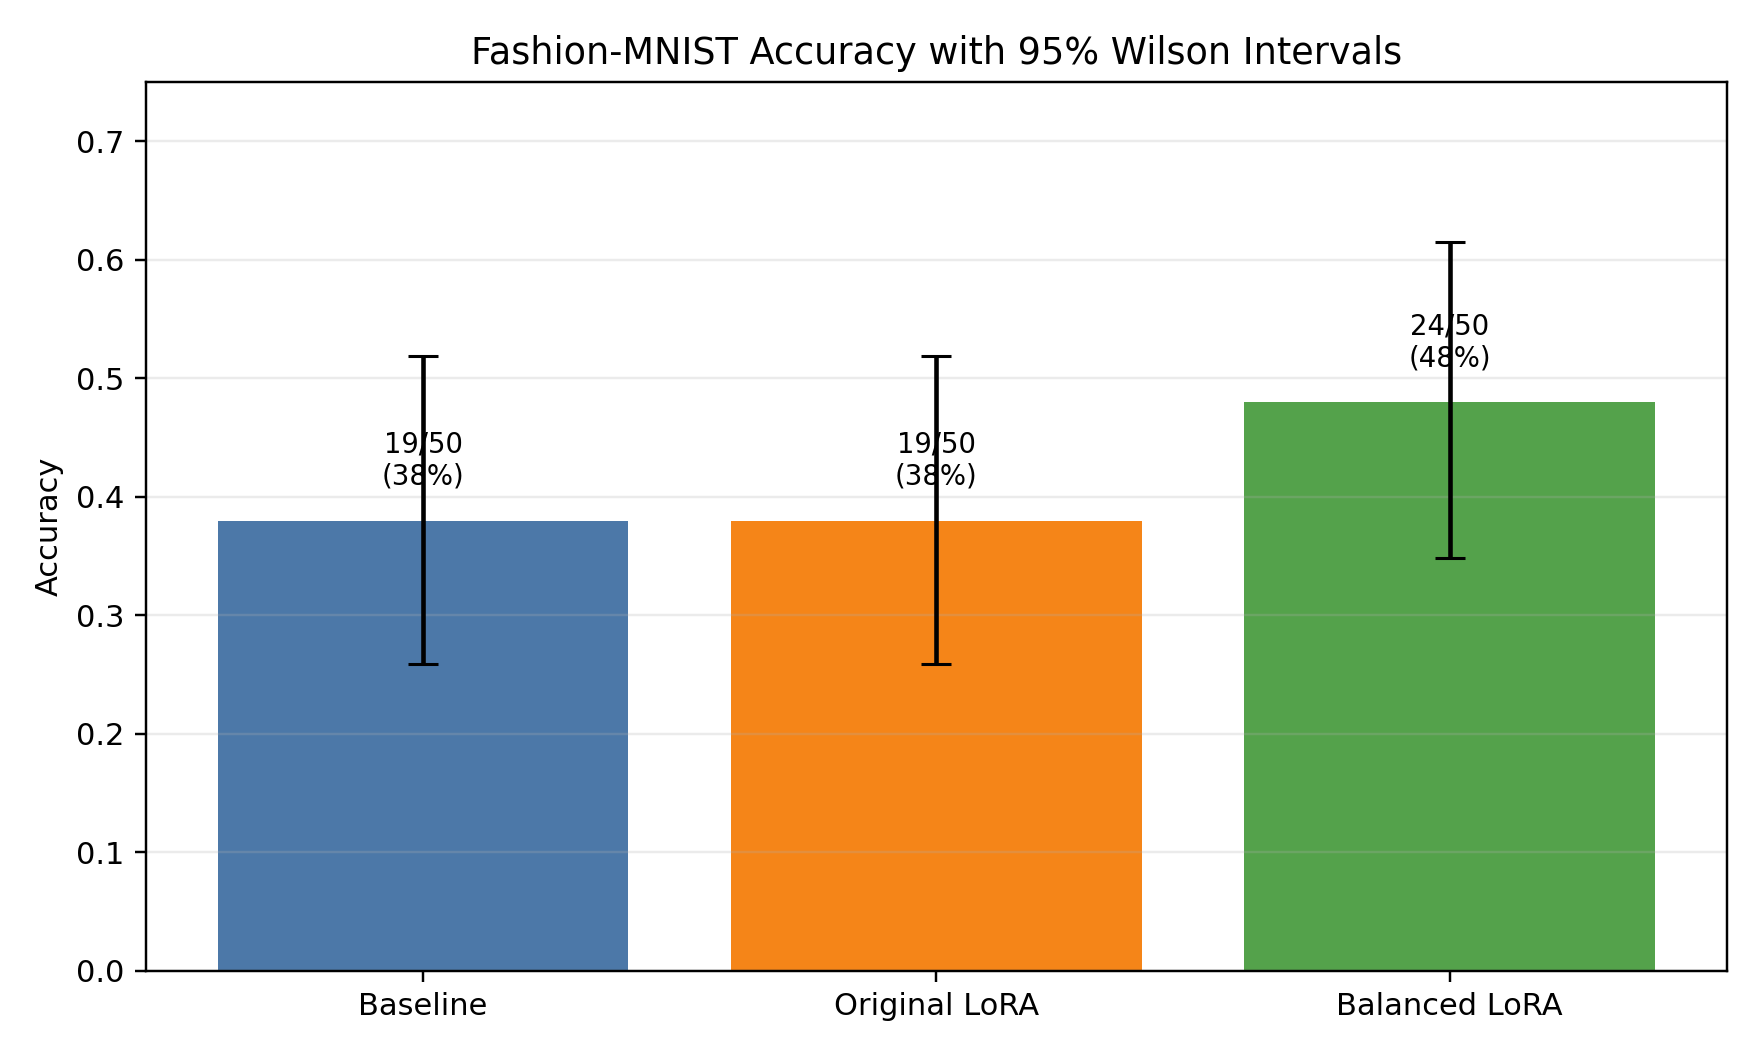
\includegraphics[width=0.78\textwidth]{accuracy_comparison.png}
\caption{Accuracy for the baseline and two LoRA adapters. The wide and
overlapping intervals reflect the limited 50-image evaluation sample.}
\label{fig:finetuned-accuracy}
\end{figure}

\section{Paired Statistical Comparison}

\begin{table}[H]
\centering
\small
\resizebox{\textwidth}{!}{%
\begin{tabular}{@{}lrrrrrr@{}}
\toprule
\textbf{Candidate} &
\textbf{Both right} &
\textbf{Fixed} &
\textbf{Regressed} &
\textbf{Both wrong} &
\textbf{McNemar \(p\)} &
\textbf{Bootstrap 95\% CI} \\
\midrule
Original LoRA
& 12 & 7 & 7 & 24 & 1.000 & [-0.14, 0.14] \\
Balanced LoRA
& 14 & 10 & 5 & 21 & 0.302 & [-0.04, 0.24] \\
\bottomrule
\end{tabular}
}
\caption{Paired comparisons against the baseline. ``Fixed'' denotes a baseline
error corrected by the adapter; ``regressed'' denotes a baseline success made
incorrect by the adapter. Bootstrap intervals describe the change in accuracy.}
\label{tab:finetuned-paired}
\end{table}

The original adapter fixes and regresses on seven examples, producing no net
gain. The balanced adapter fixes ten and regresses on five. Its effect is
promising but inconclusive: McNemar's \(p=0.302\), and the paired bootstrap
95\% interval is \([-0.04,0.24]\). It beats the baseline in 88.4\% of bootstrap
resamples, but a larger test is needed for a reliable claim.

\section{Class-Level Behaviour}

\begin{longtable}{@{}clrrr@{}}
\caption{Per-class recall. Class numbers are also used in the confusion-matrix
figure.}\label{tab:finetuned-class-recall}\\
\toprule
\textbf{Index} & \textbf{Class} & \textbf{Baseline} &
\textbf{Original LoRA} & \textbf{Balanced LoRA} \\
\midrule
\endfirsthead
\toprule
\textbf{Index} & \textbf{Class} & \textbf{Baseline} &
\textbf{Original LoRA} & \textbf{Balanced LoRA} \\
\midrule
\endhead
0 & T-shirt/top & 0.667 & 0.000 & 0.000 \\
1 & Trouser     & 0.000 & 0.143 & 0.286 \\
2 & Pullover    & 0.667 & 0.000 & 0.167 \\
3 & Dress       & 0.200 & 0.200 & 0.200 \\
4 & Coat        & 0.000 & 0.400 & 0.400 \\
5 & Sandal      & 0.000 & 0.000 & 0.250 \\
6 & Shirt       & 0.400 & 1.000 & 1.000 \\
7 & Sneaker     & 1.000 & 1.000 & 1.000 \\
8 & Bag         & 0.500 & 0.750 & 0.750 \\
9 & Ankle boot  & 0.250 & 0.000 & 0.500 \\
\bottomrule
\end{longtable}

The balanced adapter improves six classes but loses ground on T-shirt/top and
pullover. Shirt recall rises from 0.40 to 1.00, yet precision is only 0.20
because it predicts \emph{shirt} 25 times for five true shirts. The original
adapter is more concentrated still, predicting \emph{shirt} 29 times.

\begin{figure}[H]
\centering
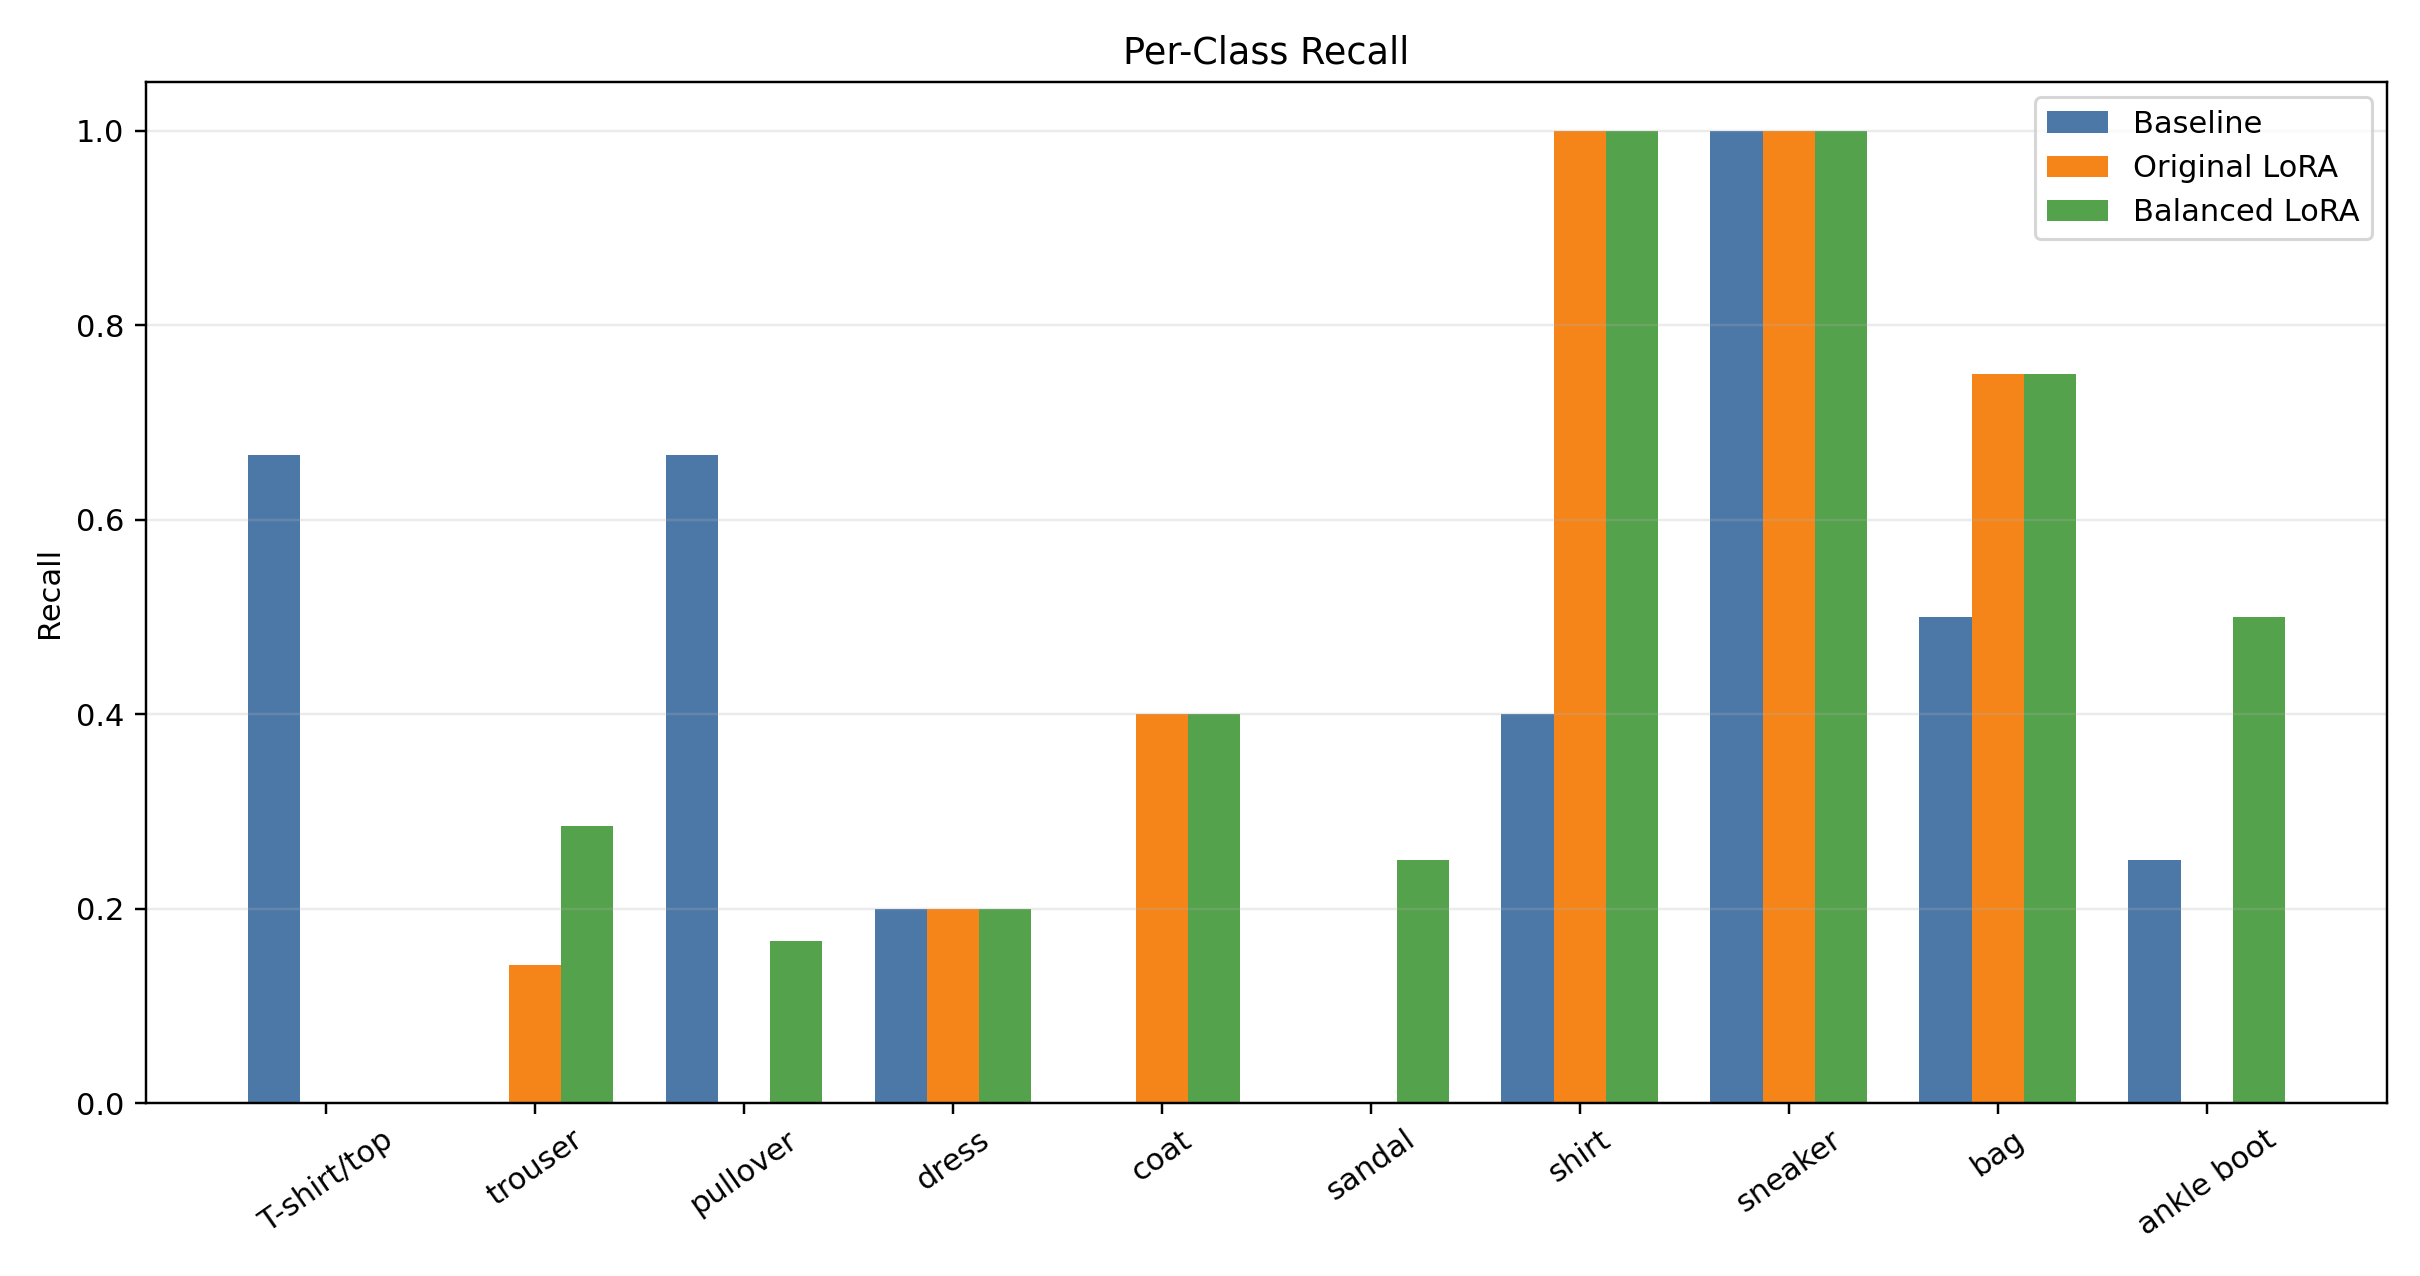
\includegraphics[width=\textwidth]{per_class_recall.png}
\caption{Recall by Fashion-MNIST class. The balanced adapter improves several
previously weak classes but loses all three T-shirt/top examples and most
pullover examples.}
\label{fig:finetuned-recall}
\end{figure}

\begin{figure}[H]
\centering
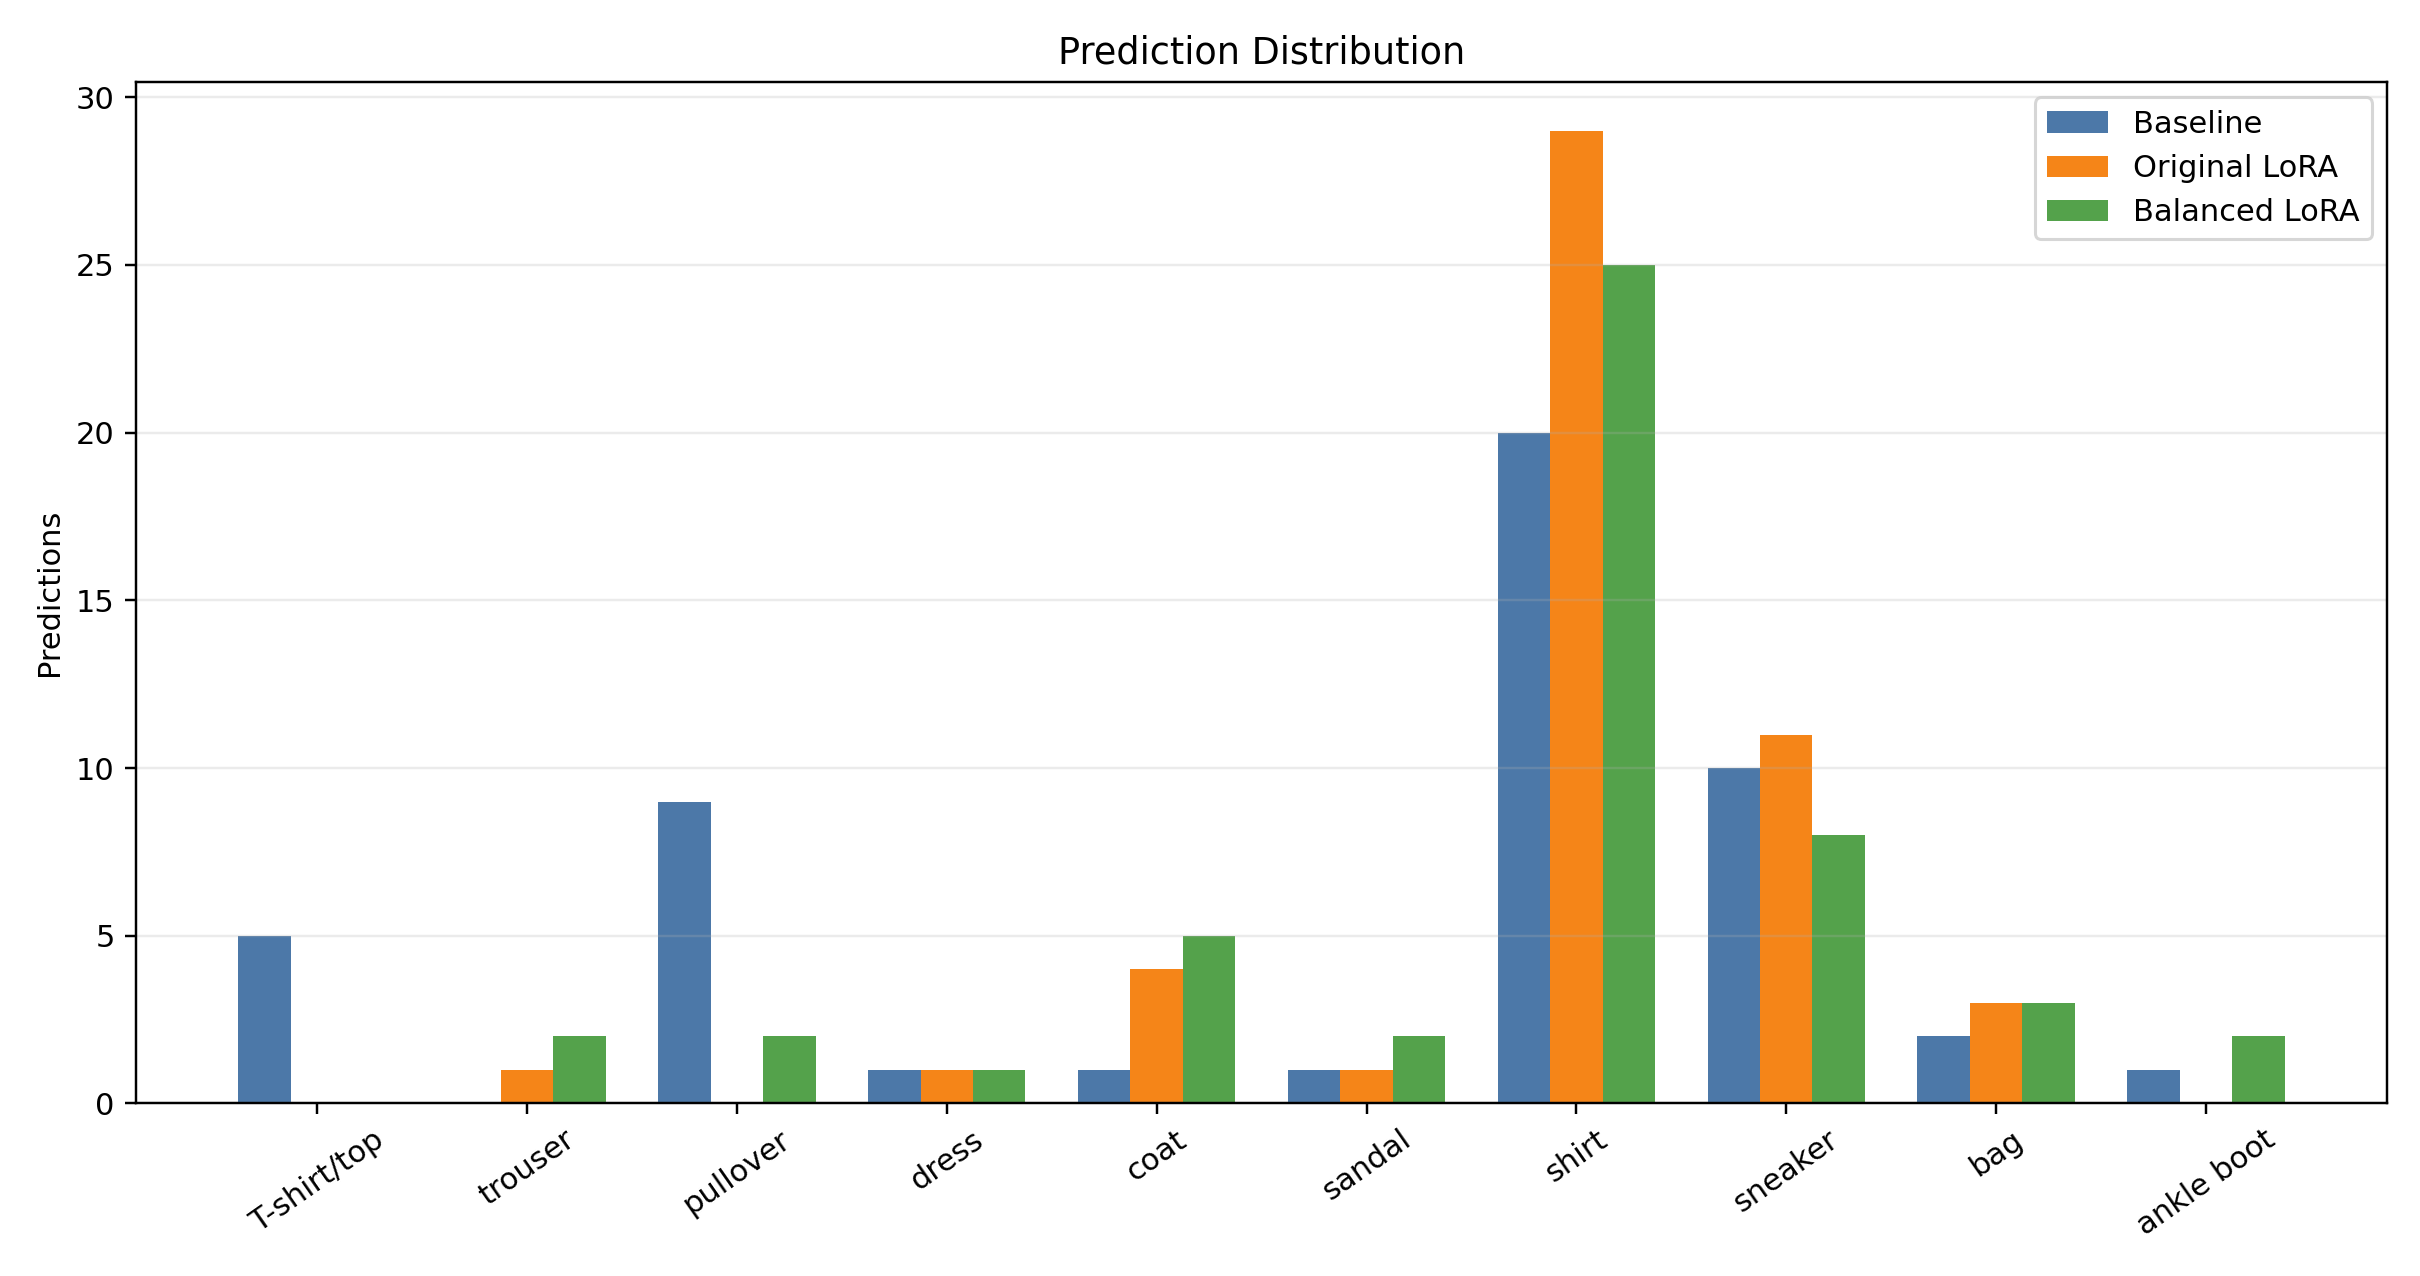
\includegraphics[width=\textwidth]{prediction_distribution.png}
\caption{Prediction frequencies. Both adapters increase the existing tendency
to predict \emph{shirt}; the original adapter exhibits the strongest
concentration.}
\label{fig:finetuned-predictions}
\end{figure}

\begin{figure}[H]
\centering
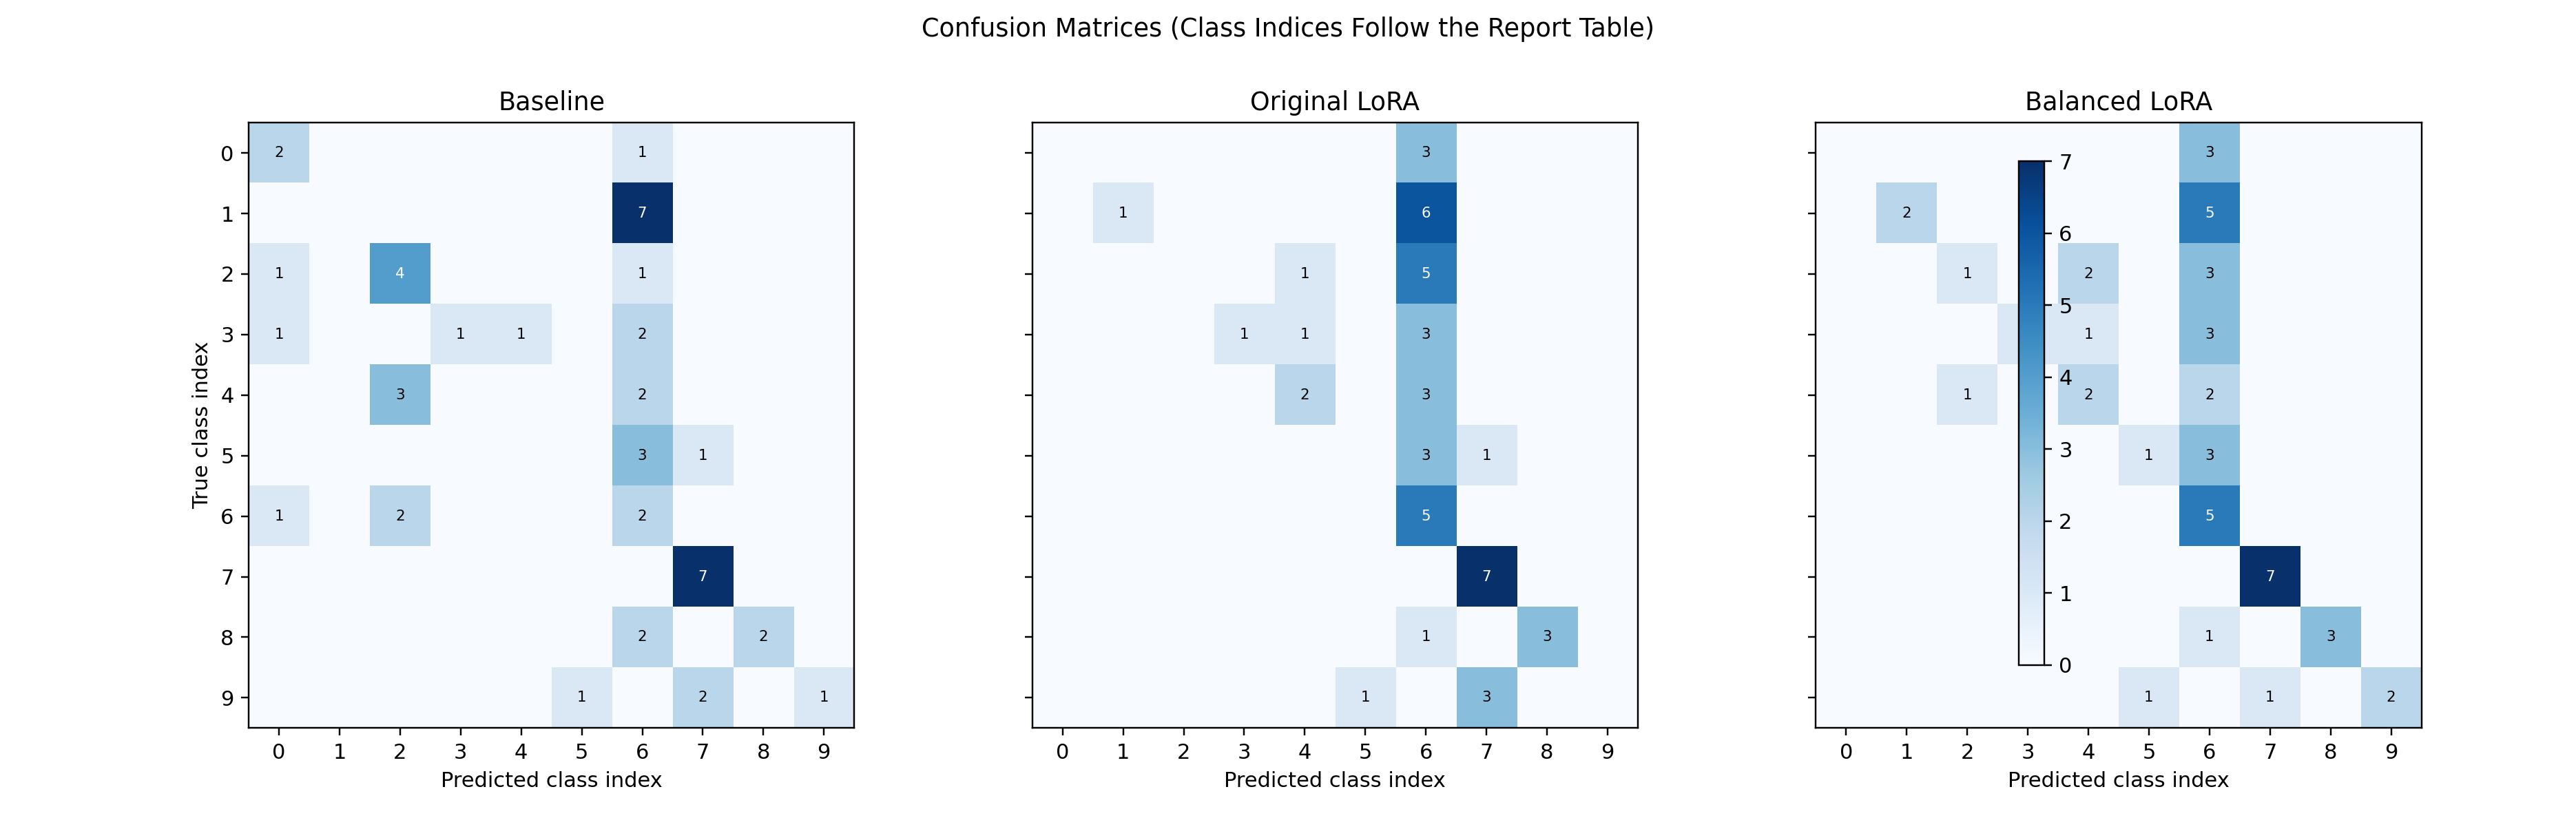
\includegraphics[width=\textwidth]{confusion_matrices.png}
\caption{Confusion matrices for the common 50-image sample. Rows are reference
classes and columns are predicted classes, using the indices in
Table~\ref{tab:finetuned-class-recall}.}
\label{fig:finetuned-confusions}
\end{figure}

\section{Inference Efficiency}

\begin{table}[H]
\centering
\small
\begin{tabular}{@{}lrrrrr@{}}
\toprule
\textbf{Model} &
\textbf{Total (s)} &
\textbf{s/sample} &
\textbf{Generation (s)} &
\textbf{Samples/s} &
\textbf{Peak VRAM (GiB)} \\
\midrule
Baseline      & 28.99 & 0.580 & 0.547 & 1.725 & 7.010 \\
Original LoRA & 31.82 & 0.636 & 0.611 & 1.571 & 7.038 \\
Balanced LoRA & 30.39 & 0.608 & 0.581 & 1.645 & 7.038 \\
\bottomrule
\end{tabular}
\caption{Measured inference telemetry for the 50-image runs. Generation time is
the mean per sample.}
\label{tab:finetuned-runtime}
\end{table}

The balanced adapter adds about 4.8\% latency per image and 0.028~GiB peak
VRAM while producing five additional correct answers. Timing differences are
less controlled than accuracy because the models were run separately.

\section{Limitations}

\begin{itemize}[leftmargin=*]
    \item Only 50 images were tested, with three to seven examples per class.
    \item Results come from one training and inference run per adapter.
    \item The findings are specific to Fashion-MNIST and do not measure general
    vision-language performance or forgetting.
\end{itemize}

\section{Conclusion}

The original LoRA provides no improvement. Balanced QLoRA raises observed
accuracy from 38\% to 48\% and macro F1 from 0.342 to 0.455 with little runtime
overhead. Because the paired interval includes zero and McNemar's test is not
significant, this is evidence of a promising sample-level gain rather than a
conclusive general improvement.

\end{document}
